%%%%%%%%%%%%%%%%%%%%%%%%%%%%%%%%%%%%%%%
% Wenneker Resume/CV
% LaTeX Template
% Version 1.1 (19/6/2016)
%
% This template has been downloaded from:
% http://www.LaTeXTemplates.com
%
% Original author:
% Frits Wenneker (http://www.howtotex.com) with extensive modifications by 
% Vel (vel@LaTeXTemplates.com)
%
% License:
% CC BY-NC-SA 3.0 (http://creativecommons.org/licenses/by-nc-sa/3.0/
%
%%%%%%%%%%%%%%%%%%%%%%%%%%%%%%%%%%%%%%

%----------------------------------------------------------------------------------------
%	PACKAGES AND OTHER DOCUMENT CONFIGURATIONS
%----------------------------------------------------------------------------------------

\documentclass[a4paper,12pt]{memoir} % Font and paper size

%%%%%%%%%%%%%%%%%%%%%%%%%%%%%%%%%%%%%%%%%
% Wenneker Resume/CV
% Structure Specification File
% Version 1.1 (19/6/2016)
%
% This file has been downloaded from:
% http://www.LaTeXTemplates.com
%
% Original author:
% Frits Wenneker (http://www.howtotex.com) with extensive modifications by 
% Vel (vel@latextemplates.com)
%
% License:
% CC BY-NC-SA 3.0 (http://creativecommons.org/licenses/by-nc-sa/3.0/)
%
%%%%%%%%%%%%%%%%%%%%%%%%%%%%%%%%%%%%%%%%%

%----------------------------------------------------------------------------------------
%	PACKAGES AND OTHER DOCUMENT CONFIGURATIONS
%----------------------------------------------------------------------------------------

\usepackage{XCharter} % Use the Bitstream Charter font
\usepackage[utf8]{inputenc} % Required for inputting international characters
\usepackage[T1]{fontenc} % Output font encoding for international characters

\usepackage[top=1cm,left=1cm,right=1cm,bottom=1cm]{geometry} % Modify margins

\usepackage{graphicx} % Required for figures

\usepackage{flowfram} % Required for the multi-column layout

\usepackage{url} % URLs

\usepackage[usenames,dvipsnames]{xcolor} % Required for custom colours

\usepackage{tikz} % Required for the horizontal rule

\usepackage{enumitem} % Required for modifying lists
\setlist{noitemsep,nolistsep} % Remove spacing within and around lists

\setlength{\columnsep}{\baselineskip} % Set the spacing between columns

% Define the left frame (sidebar)
\newflowframe{0.2\textwidth}{\textheight}{0pt}{0pt}[left]
\newlength{\LeftMainSep}
\setlength{\LeftMainSep}{0.2\textwidth}
\addtolength{\LeftMainSep}{1\columnsep}
 
% Small static frame for the vertical line
\newstaticframe{1.5pt}{\textheight}{\LeftMainSep}{0pt}
 
% Content of the static frame with the vertical line
\begin{staticcontents}{1}
\hfill
\tikz{\draw[loosely dotted,color=RoyalBlue,line width=1.5pt,yshift=0](0,0) -- (0,\textheight);}
\hfill\mbox{}
\end{staticcontents}
 
% Define the right frame (main body)
\addtolength{\LeftMainSep}{1.5pt}
\addtolength{\LeftMainSep}{1\columnsep}
\newflowframe{0.7\textwidth}{\textheight}{\LeftMainSep}{0pt}[main01]

\pagestyle{empty} % Disable all page numbering

\setlength{\parindent}{0pt} % Stop paragraph indentation

%----------------------------------------------------------------------------------------
%	NEW COMMANDS
%----------------------------------------------------------------------------------------

\newcommand{\userinformation}[1]{\renewcommand{\userinformation}{#1}} % Define a new command for the CV user's information that goes into the left column

\newcommand{\cvheading}[1]{{\Huge\bfseries\color{RoyalBlue} #1} \par\vspace{.6\baselineskip}} % New command for the CV heading
\newcommand{\cvsubheading}[1]{{\Large\bfseries #1} \bigbreak} % New command for the CV subheading

\newcommand{\Sep}{\vspace{1em}} % New command for the spacing between headings
\newcommand{\SmallSep}{\vspace{0.5em}} % New command for the spacing within headings

\newcommand{\aboutme}[2]{ % New command for the about me section
\textbf{\color{RoyalBlue} #1}~~#2\par\Sep
}
	
\newcommand{\CVSection}[1]{ % New command for the headings within sections
{\Large\textbf{#1}}\par
\SmallSep % Used for spacing
}

\newcommand{\CVItem}[2]{ % New command for the item descriptions
\textbf{\color{RoyalBlue} #1}\par
#2
\SmallSep % Used for spacing
}

\newcommand{\bluebullet}{\textcolor{RoyalBlue}{$\circ$}~~} % New command for the blue bullets
 % Include the file specifying document layout and packages

%----------------------------------------------------------------------------------------
%	NAME AND CONTACT INFORMATION 
%----------------------------------------------------------------------------------------

\userinformation{ % Set the content that goes into the sidebar of each page
\begin{flushright}
% Comment out this figure block if you don't want a photo
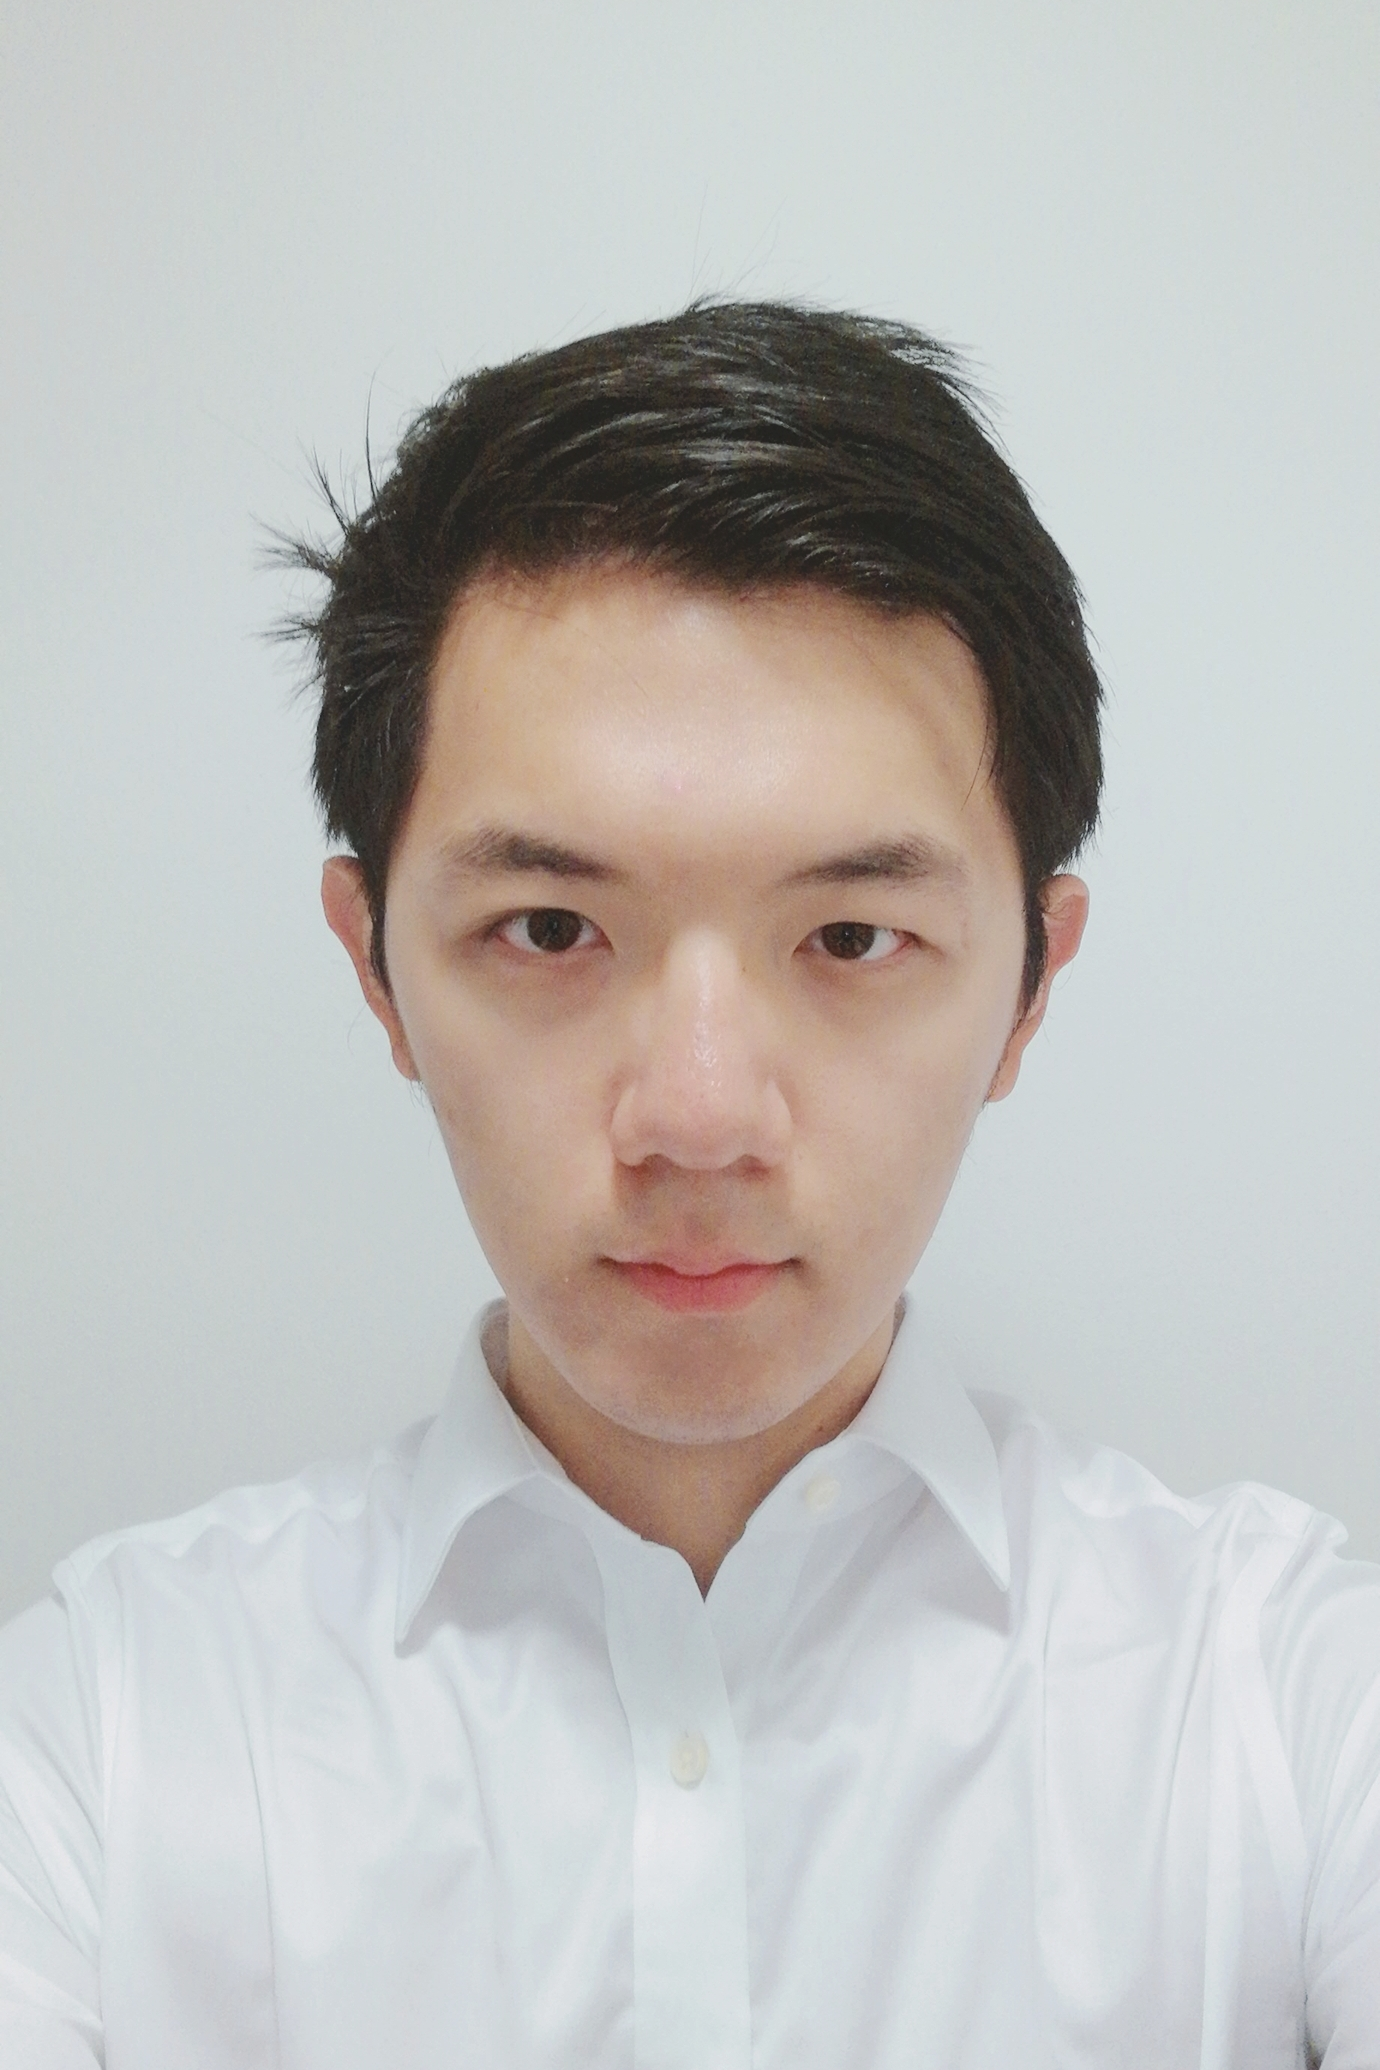
\includegraphics[width=0.6\columnwidth]{profile.jpg}\\[\baselineskip] % Your photo
\small % Smaller font size
Xiaoshen Hou \\ % Your name
\url{houxiaoshen81@gmail.com} \\ % Your email address
Age: 25 \\
Nationality: Chinese \\
(+45) 50350428 \\ % Your phone number
\Sep % Some whitespace
\textbf{Address} \\
245 Rødovre Parkvej \\ % Address 1
Rødovre 2610, Copenhagen \\ % Address 2
Denmark \\ % Address 3
\vfill % Whitespace under this block to push it up under the photo
\end{flushright}
}

%----------------------------------------------------------------------------------------

\begin{document}

\userinformation % Print your information in the left column

\framebreak % End of the first column

%----------------------------------------------------------------------------------------
%	HEADING
%----------------------------------------------------------------------------------------

\cvheading{Xiaoshen Hou} % Large heading - your name

\cvsubheading{Big Data Engineer} % Subheading - your occupation/specialization

%----------------------------------------------------------------------------------------
%	ABOUT ME
%----------------------------------------------------------------------------------------

\aboutme{About Me}{I am currently working as a big data consultant. My education and working experience so far are able to contribute and add significant amount of strength to support me in career. }

%----------------------------------------------------------------------------------------
%	EDUCATION
%----------------------------------------------------------------------------------------

\CVSection{Education}

%------------------------------------------------

\CVItem{2016 - 2018, Technical University of Denmark}{MSc in Digital Media Engineering - Studyline: Data Science}

%------------------------------------------------

\CVItem{2012 - 2016, Technical University of Denmark}{BEng in Information Technology}

%------------------------------------------------

\Sep % Extra whitespace after the end of a major section

%----------------------------------------------------------------------------------------
%	EXPERIENCE
%----------------------------------------------------------------------------------------

\CVSection{Experience}

%------------------------------------------------

\CVItem{SEP 2015 - now, \textit{Consultant of Big Data(Hadoop) Solution}, Nordea Bank Denmark, Hadoop Data Platform}{
Work Contents:
\begin{itemize}
	\item Make ETL process in Spark, manage storage in Hive/HBase and quick data retrieval such as Solr.
	\item Build Data pipeline with tools from standard Hadoop Distribution.
	\item Manage Kerberos authentication and AD controls over entire cluster
	\item Analyze and Visualize preprocessed data with Python (Jupyter) 
	\item Work in an agile development approach. Utilize Atlassian porducts and source code hosting sites bitbucket, github. 
	\item Involved in many automatic tools in enterprise level such as Puppet, Docker, Bamboo, Remedy etc.
\end{itemize}
}

%------------------------------------------------

\CVItem{FEB 2015 - AUG 2015, \textit{Web Developer Intern}, Deskwolf A/S}{Half year internship at a startup majorly working with social media especially Facebook. Developing web application hosted in CMS system in PHP as well as Javascript. The purpose is to attract and assist other offline SMEs to boost their business via social media.}

%------------------------------------------------

\Sep % Extra whitespace after the end of a major section

%----------------------------------------------------------------------------------------
%	COMMUNICATION SKILLS
%----------------------------------------------------------------------------------------

\CVSection{Language Skills}

%------------------------------------------------

\bluebullet \CVItem{Chinese (Mandarin)}{ Mother tongue} \\
\bluebullet \CVItem{English}{ Business} \\
\bluebullet \CVItem{Danish}{ Intermediate} \\

%------------------------------------------------

\Sep % Extra whitespace after the end of a major section

%----------------------------------------------------------------------------------------
%	SKILLS
%----------------------------------------------------------------------------------------

\CVSection{Programming Skills}

%------------------------------------------------

\CVItem{Programming} 
{\begin{tabular}{p{0.2\textwidth} p{0.2\textwidth} p{0.2\textwidth} p{0.2\textwidth}}
\bluebullet Java (Maven) &  \bluebullet Python & \bluebullet Shell & \bluebullet SQL \\
\bluebullet JS & \bluebullet Matlab \\
\end{tabular}}

%------------------------------------------------

\CVItem{Enterprise Solutions}
{\begin{tabular}{p{0.2\textwidth} p{0.2\textwidth} p{0.2\textwidth} p{0.2\textwidth}}
 \bluebullet Cloudera Hadoop &  \bluebullet Anaconda & \bluebullet Agile & \bluebullet Kafka &  \bluebullet Bitbucket(Git) & \bluebullet Puppet 
\end{tabular}}

%------------------------------------------------

\Sep % Extra whitespace after the end of a major section

%----------------------------------------------------------------------------------------
%	NEW PAGE DELIMITER
%	Place this block wherever you would like the content of your CV to go onto the next page
%----------------------------------------------------------------------------------------

\clearpage % Start a new page

\userinformation % Print your information in the left column

\framebreak % End of the first column

%----------------------------------------------------------------------------------------
%	AWARDS
%----------------------------------------------------------------------------------------

\CVSection{Awards}

%------------------------------------------------

\CVItem{2016, \textit{Postgraduate Degree Tuition Fee Waiver},Technical University of Denmark}{Tuition fee waiver awarded to the top student from outside of EU countries in a postgraduate degree.} 

\CVItem{2012, \textit{Undergraduate Scholarship and Tuition Fee Waiver},Technical University of Denmark}{Scholarship and tuition fee waiver awarded to the top student from outside of EU countries during undergraduate study.} 


%------------------------------------------------
\Sep 
\CVSection{GPAs}

%------------------------------------------------

\CVItem{Master : 11/12}
\small{Link:https://cn.inside.dtu.dk/cnnet/Grades/Public.aspx?Id=UDZ5T58PM3} 

\CVItem{Bachelor : 11.7/12}
\small{Link:https://cn.inside.dtu.dk/cnnet/Grades/Public.aspx?Id=SVFJCSZ7VZ} 

%------------------------------------------------

\Sep % Extra whitespace after the end of a major section

%----------------------------------------------------------------------------------------
%	Projects
%----------------------------------------------------------------------------------------

\CVSection{Projects}

\textit{Github profile:https://github.com/ShawnHouCHN} \\

%------------------------------------------------

\CVItem{1. (Network Science) - Discover the hidden communities of enterprises.}{ Project Webpage: \\ \small{https://shawnhouchn.github.io/Social-Graph-Interaction/project/WolfOfMatematiktorvet/}}

\CVItem{2. (Machine Learning) - NYC Car Accident Analysis}{ Project Webpage: \\ \small{https://shawnhouchn.github.io/SDAV2017-Project/Web/}}

\CVItem{3. (Machine Learning) - Primer League Match Prediction Challenge}{ Project Notebooks: \\ \small{https://github.com/ShawnHouCHN/Introduction-to-Machine-Learning-and-Data-Mining-E17}}

\CVItem{4. (Machine Learning) - Large-Scale Social Media Data Used as Sensor for Weather Change}{ Project Notebooks: \\ \small{https://github.com/ShawnHouCHN/Large-scale-social-media-data-as-a-sensor-for-public-opinion-on-climate-change}}

%------------------------------------------------


\Sep % Extra whitespace after the end of a major section

%----------------------------------------------------------------------------------------

\end{document}

